\begin{figure}[htp] \centering
    \begin{subfigure}[b]{0.5\columnwidth}
        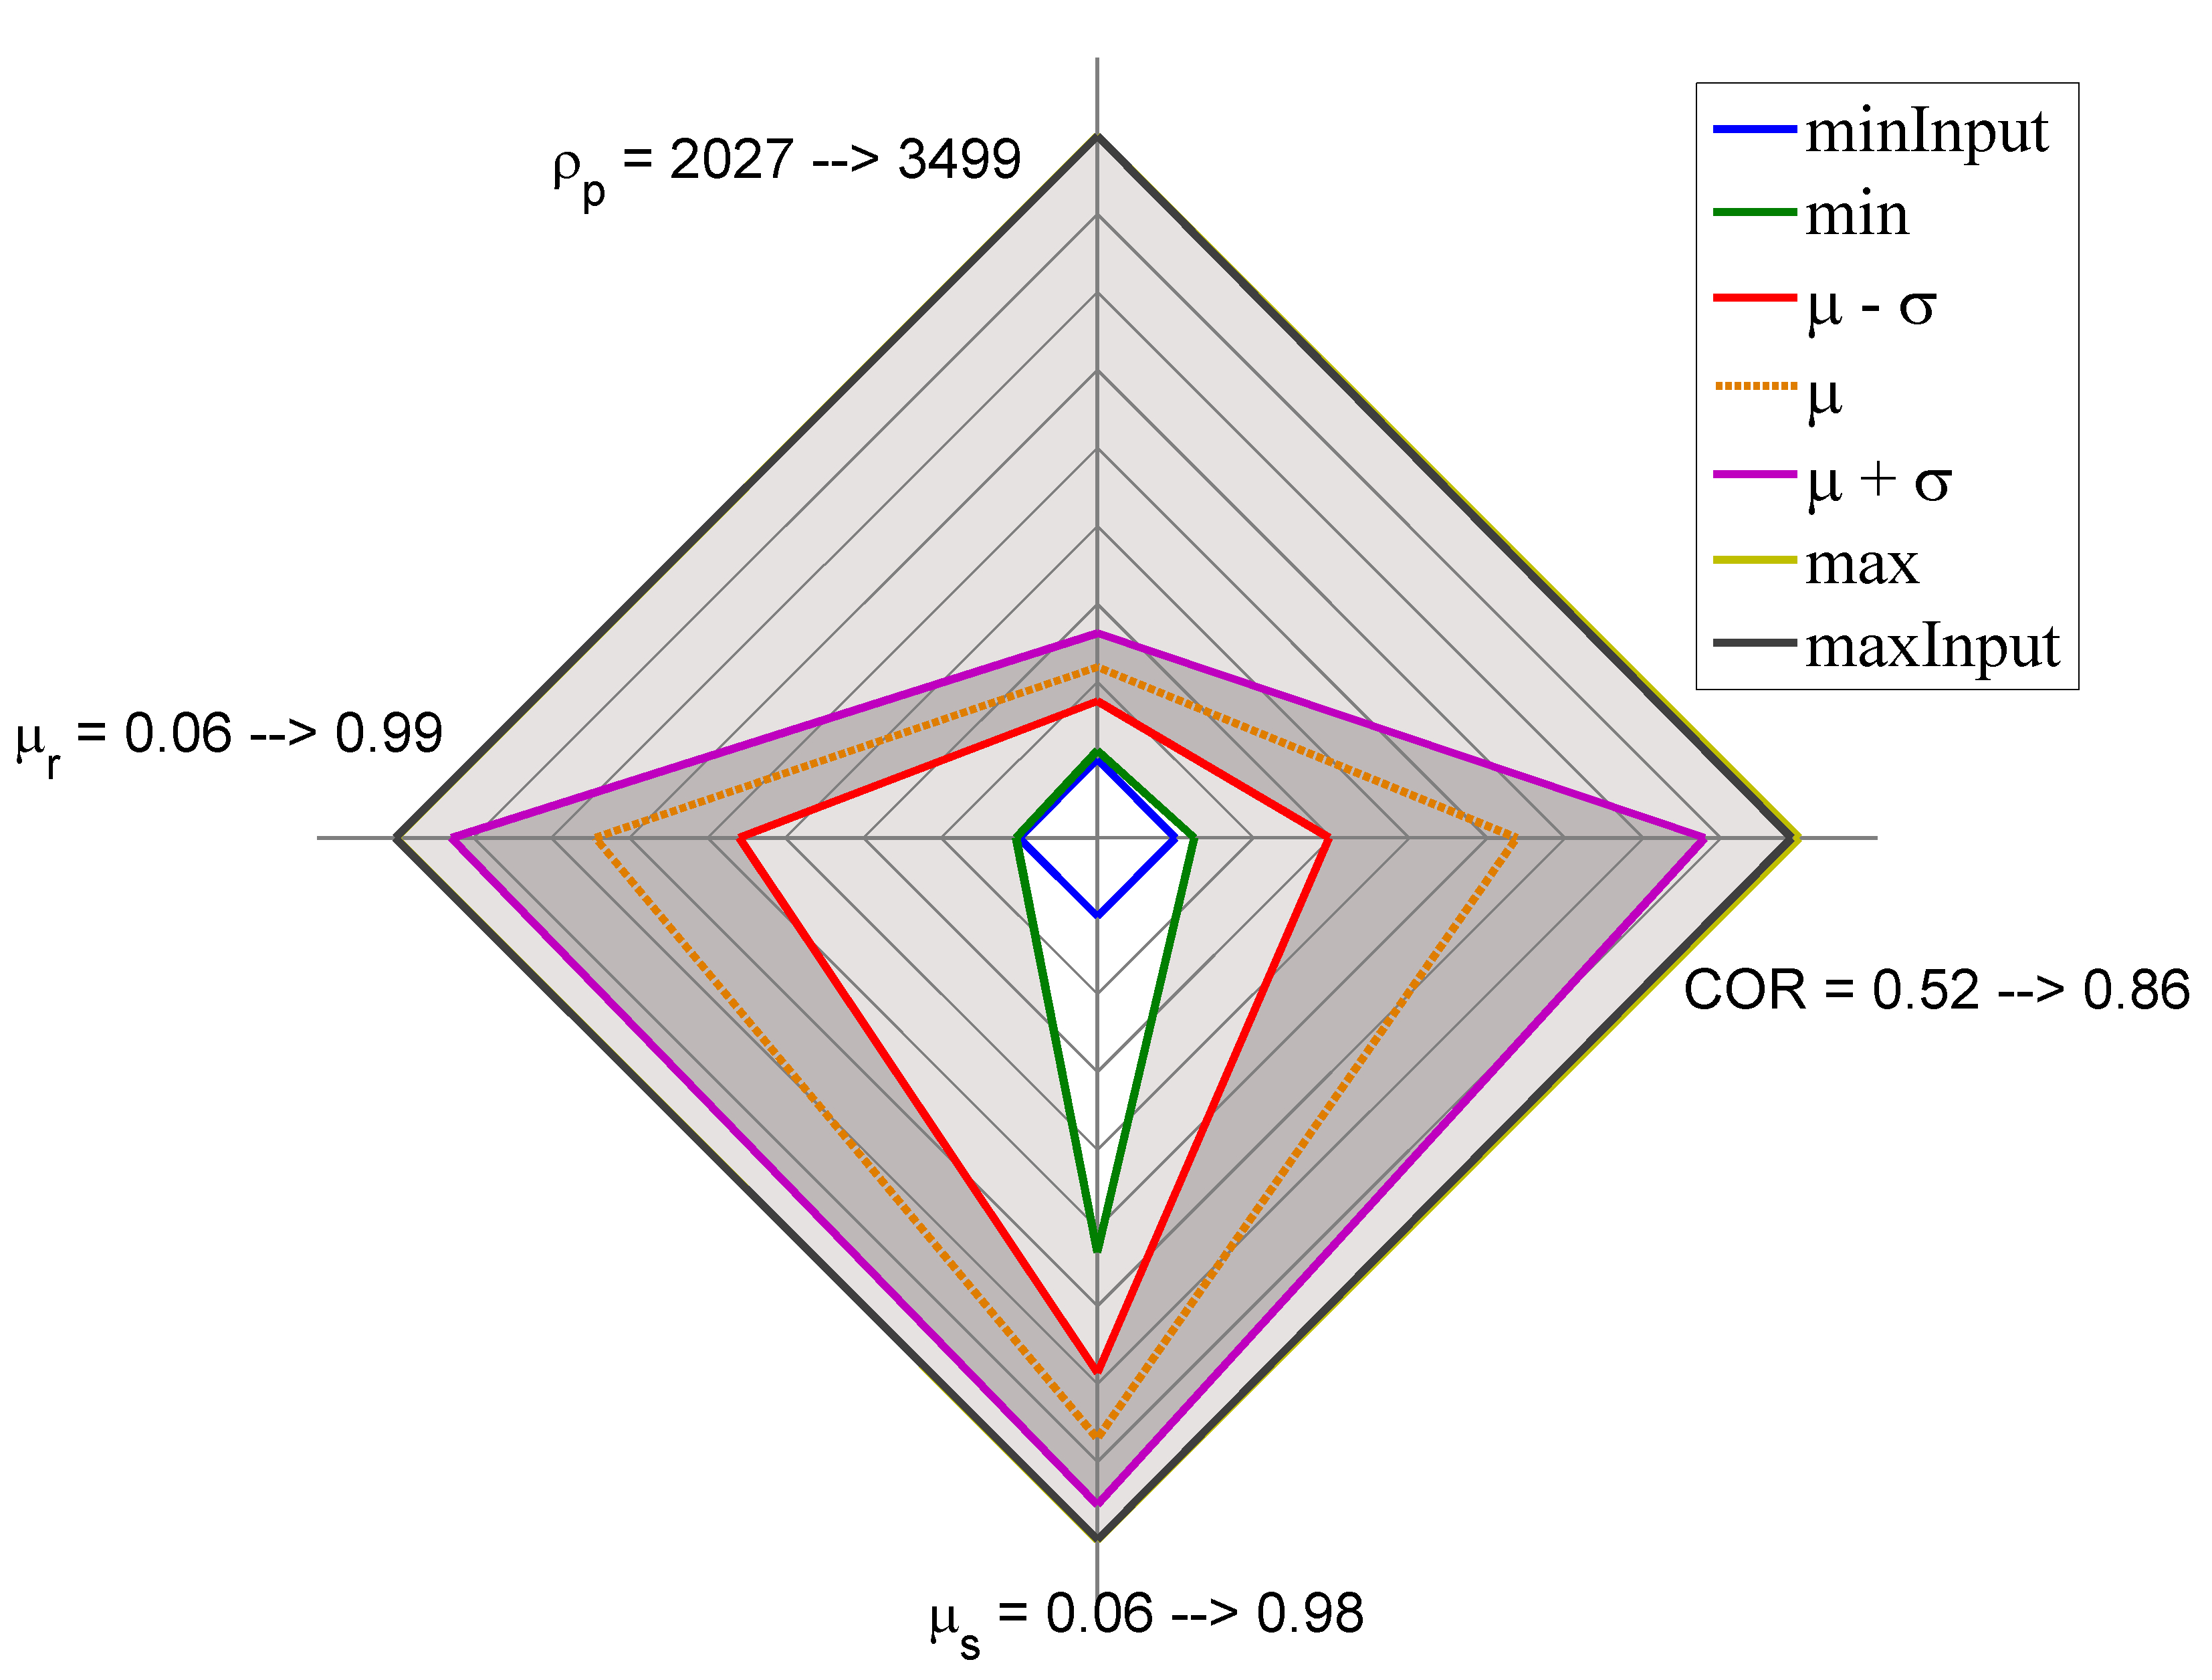
\includegraphics[width=\textwidth]{images/original/24radarpirker1schulze10070}
        \caption{Radar plot, $SCT$, $\sigma_n=10070 ~[Pa]$, $P=1.0$}
        \label{fig:24radarpirker1schulze10070}
    \end{subfigure} \\
        \begin{subfigure}[b]{0.5\columnwidth}
        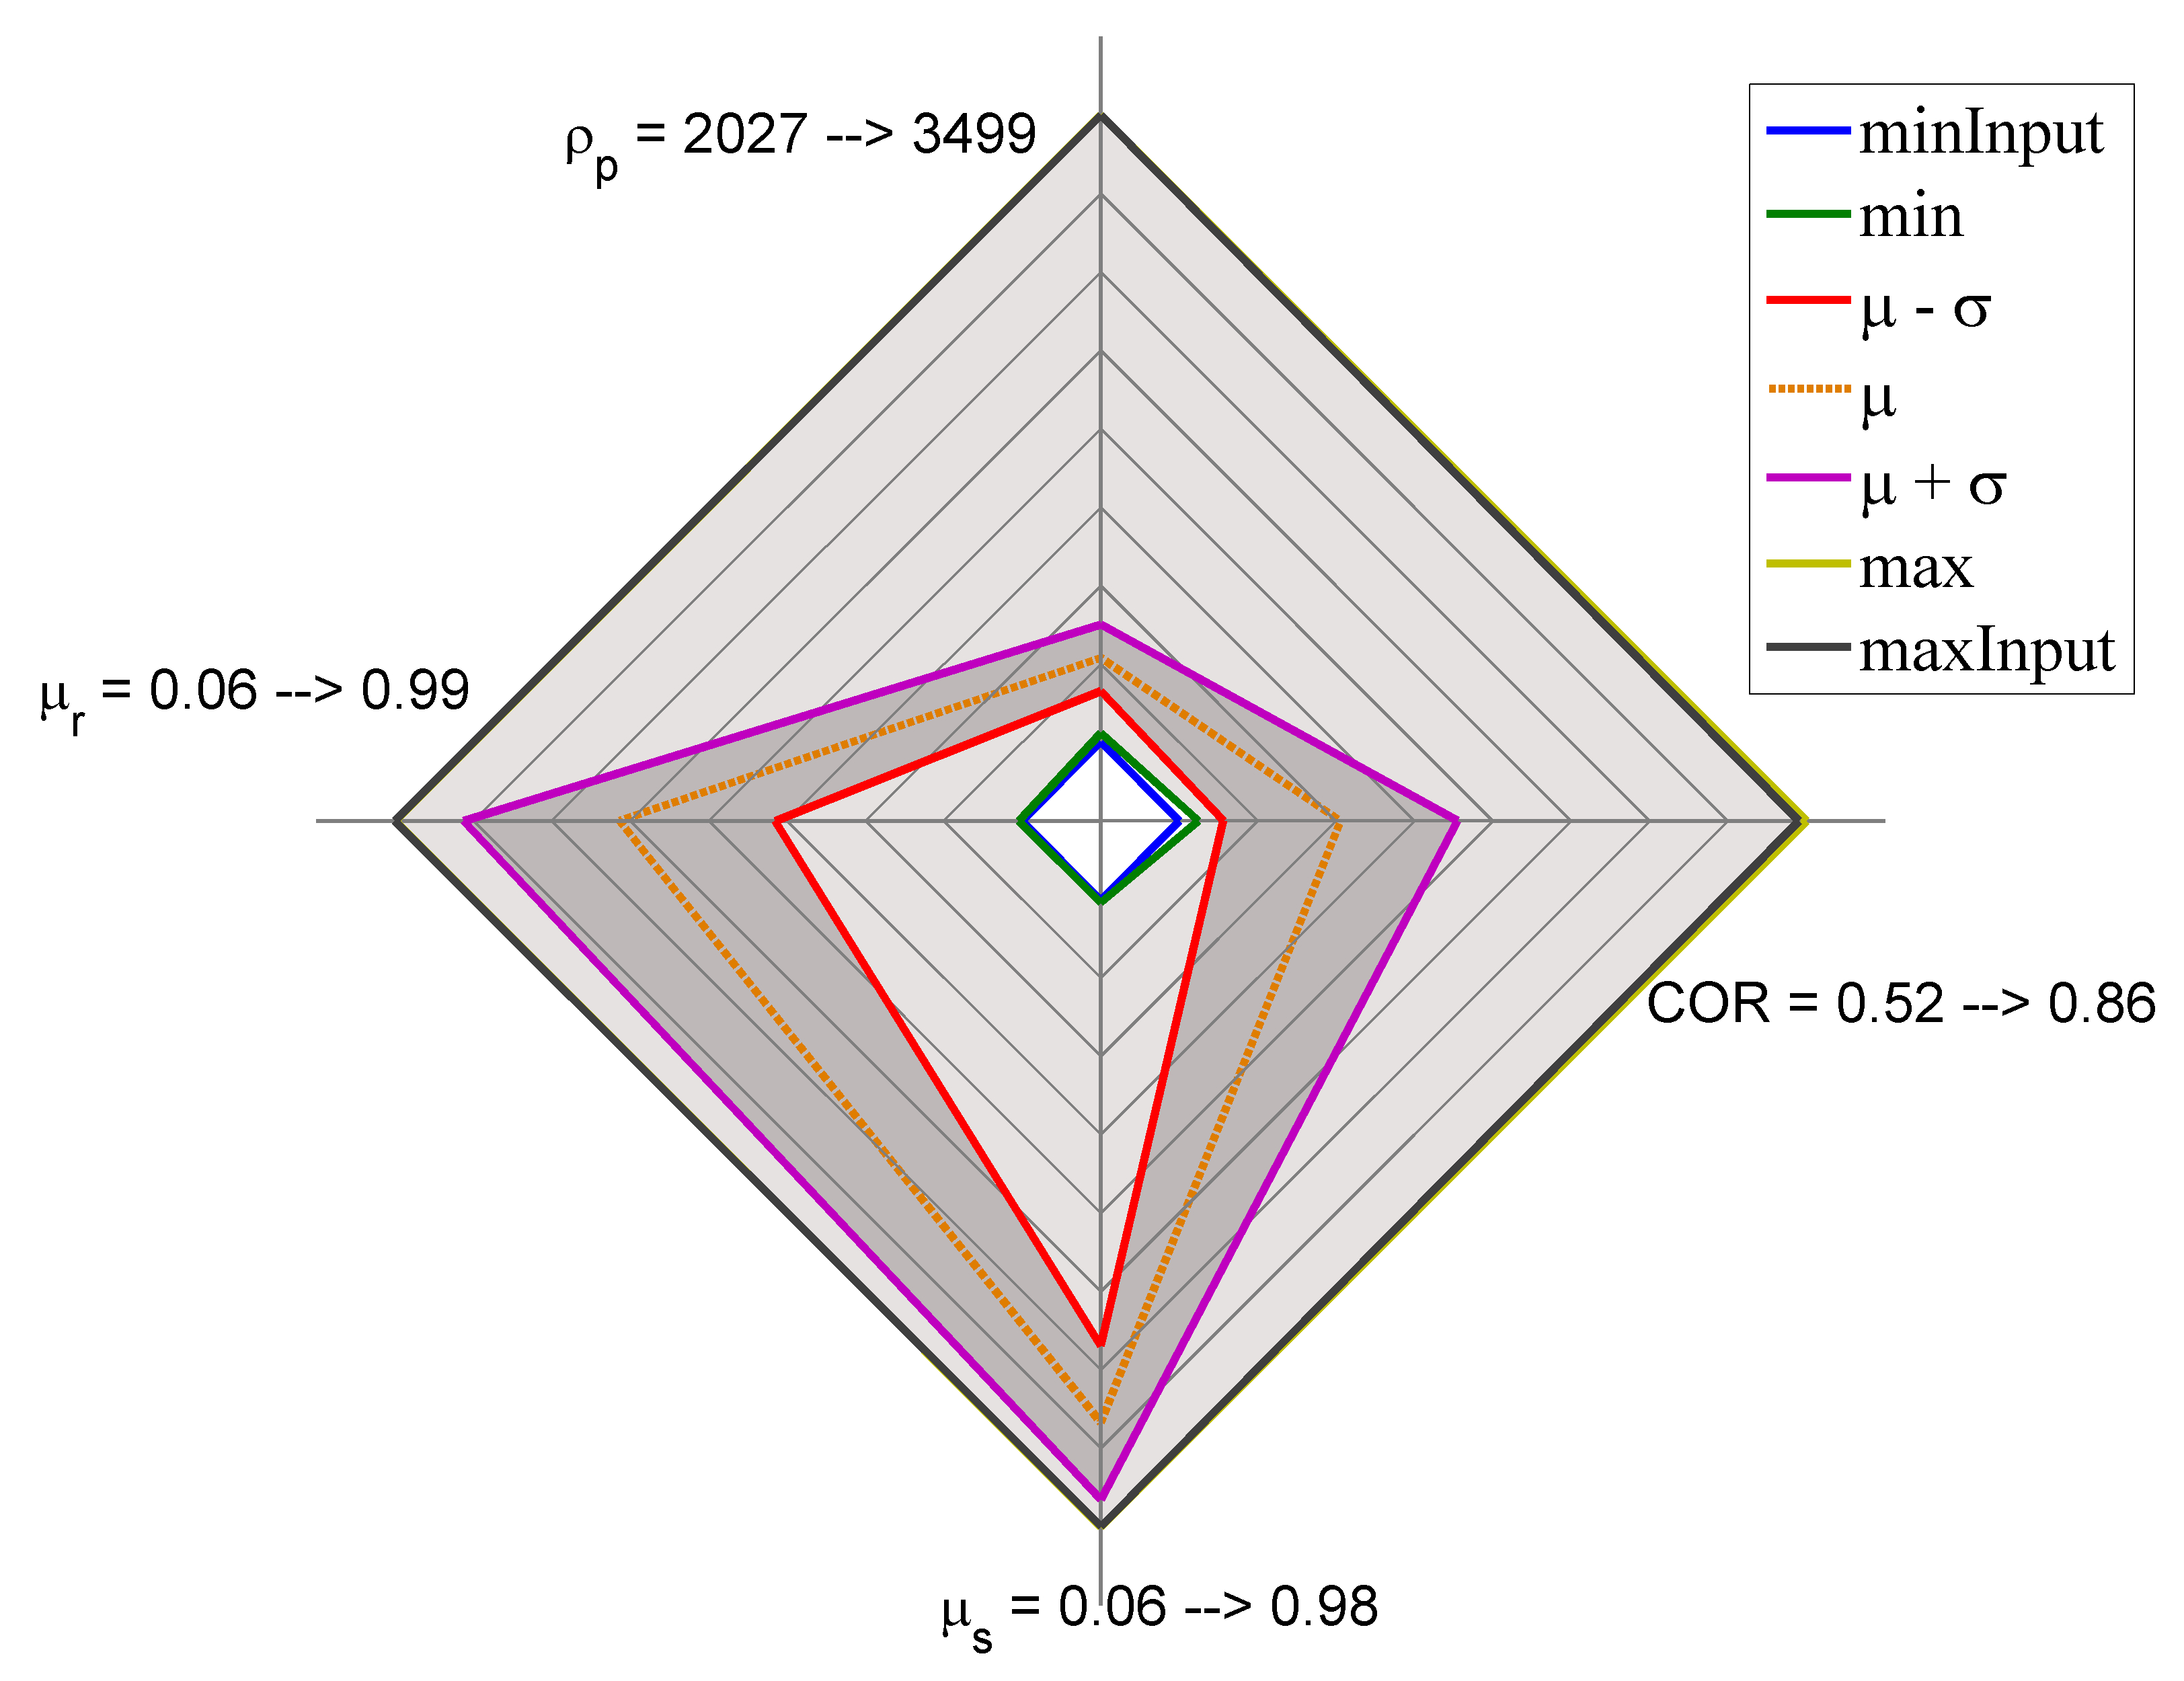
\includegraphics[width=\textwidth]{images/original/26radarpirker08schulze10070}
        \caption{Radar plot, $SCT$, $\sigma_n=10070 ~[Pa]$, $P=0.8$}
        \label{fig:26radarpirker08schulze10070} 
    \end{subfigure}\\
        \begin{subfigure}[b]{0.5\columnwidth}
        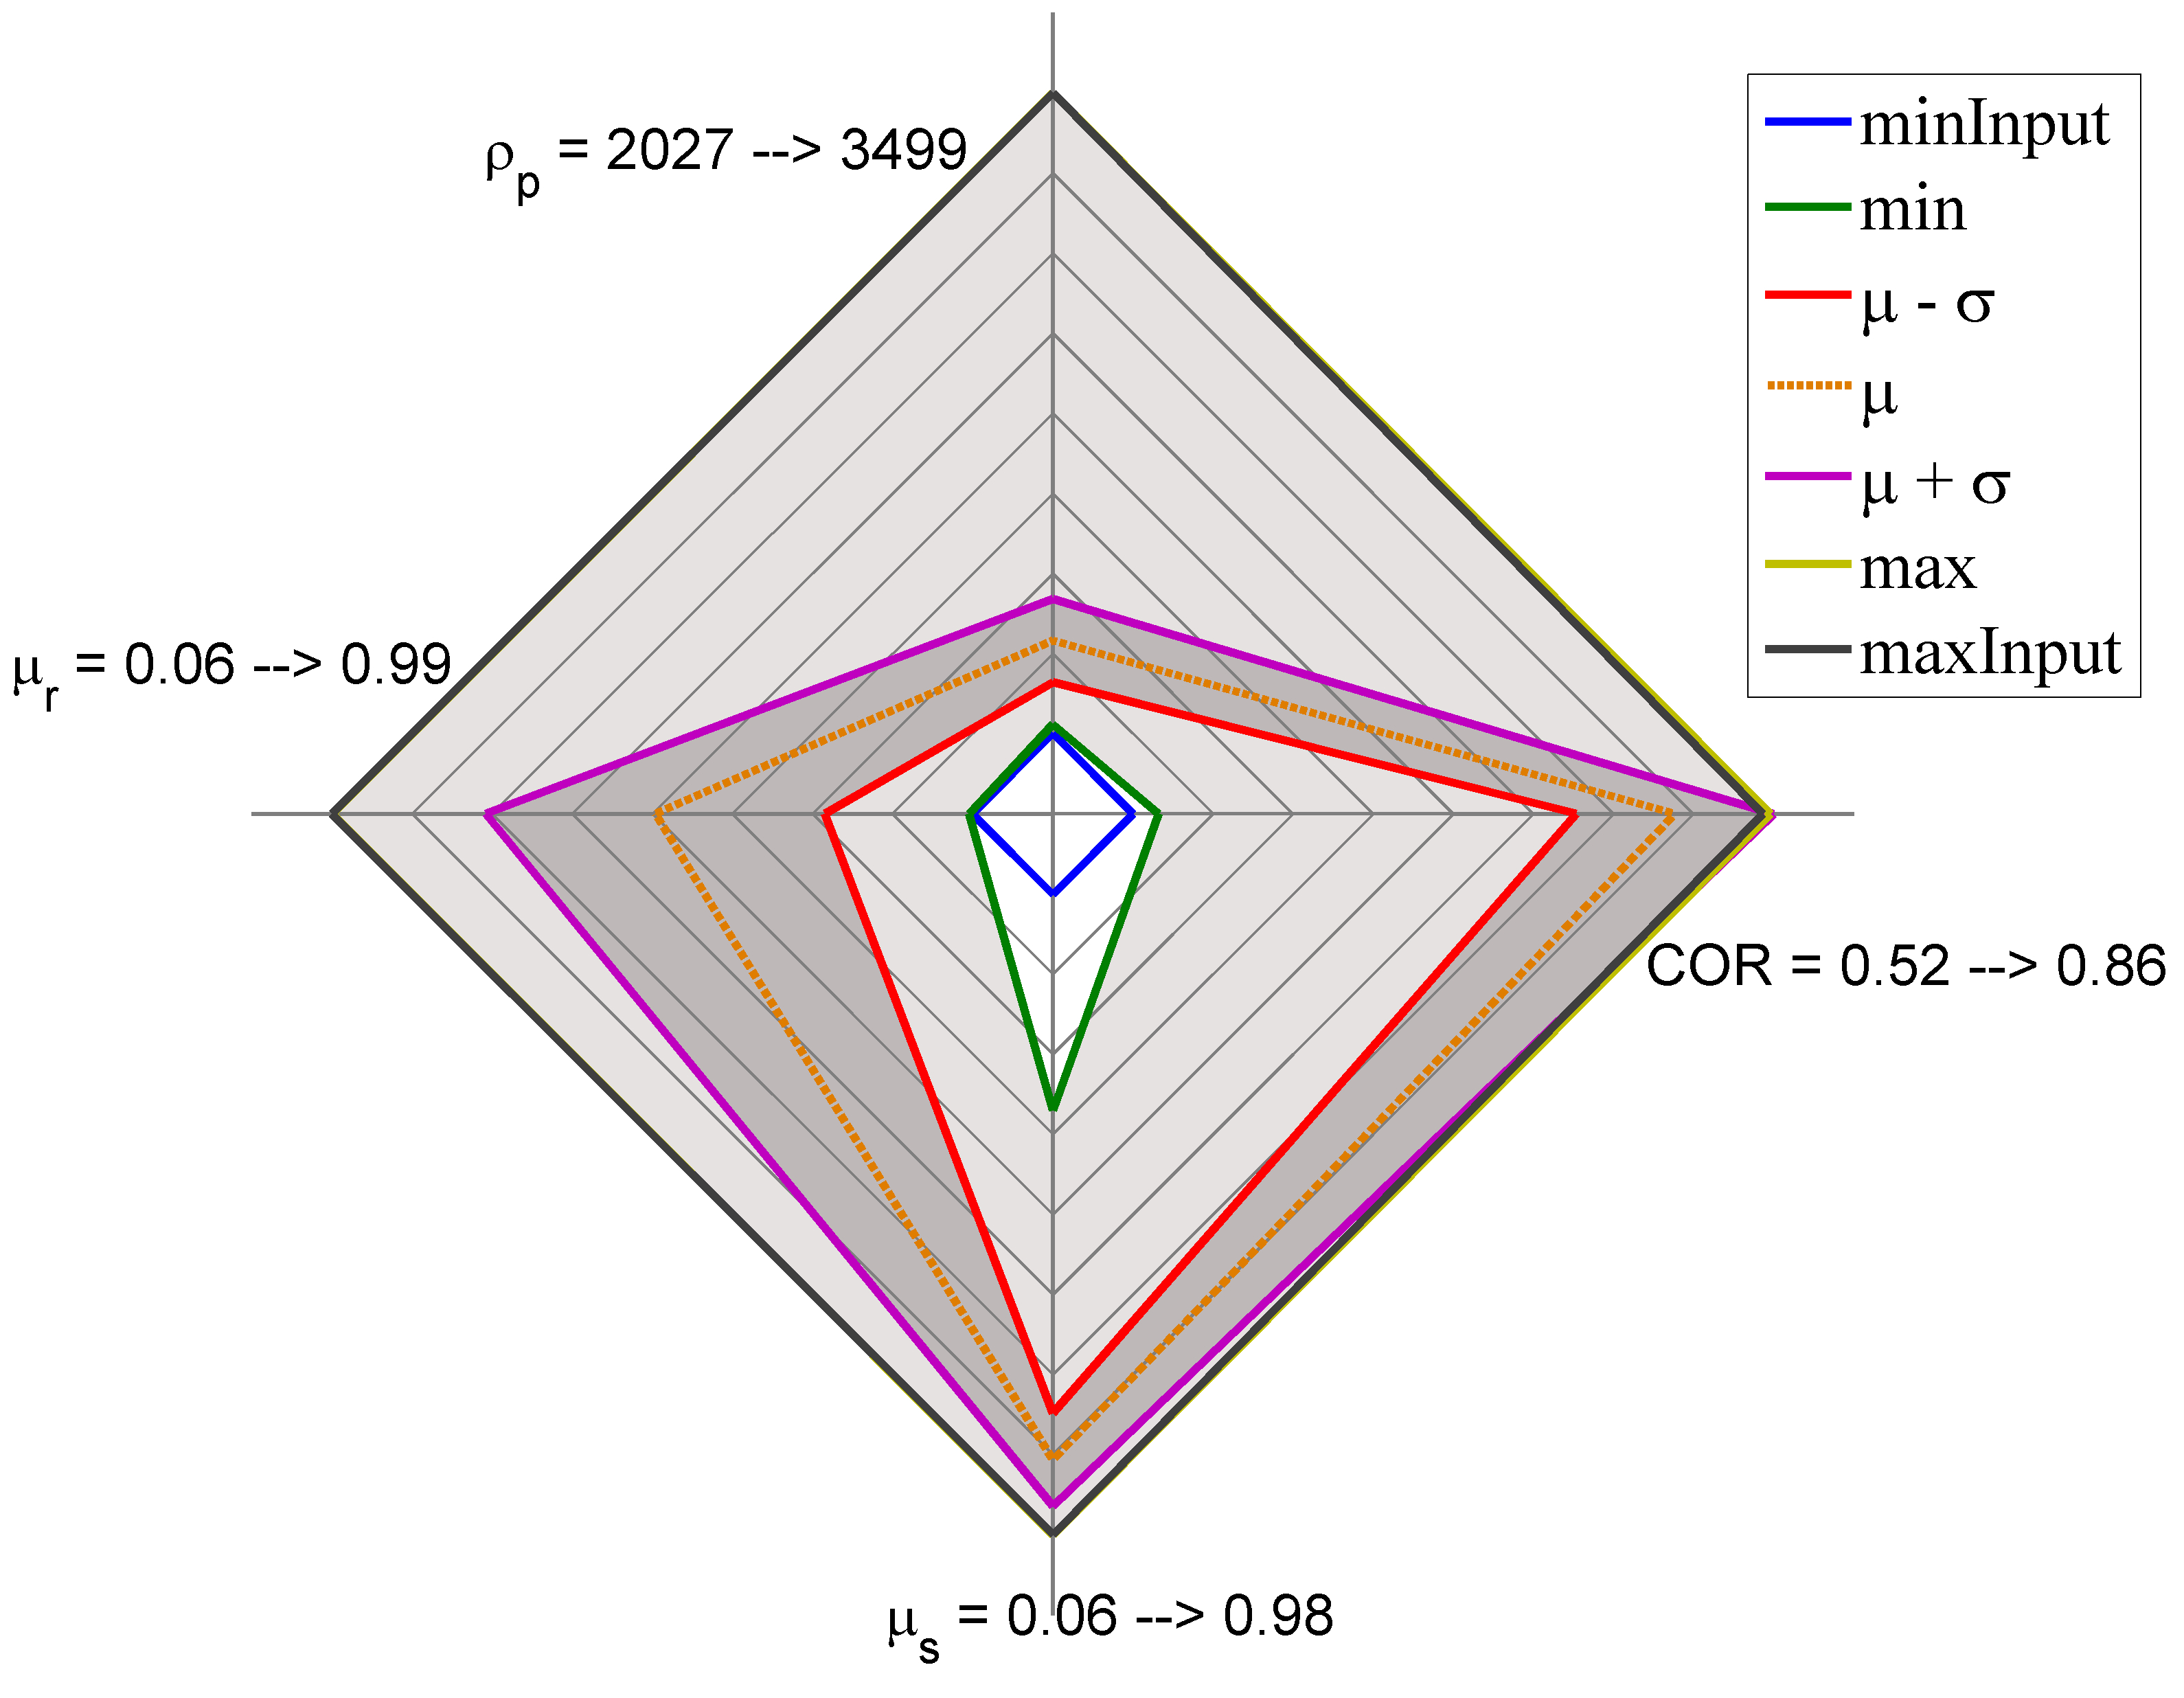
\includegraphics[width=\textwidth]{images/original/28radarpirker12schulze10070}
        \caption{Radar plot, $SCT$, $\sigma_n=10070 ~[Pa]$, $P=1.2$}
        \label{fig:28radarpirker12schulze10070} 
    \end{subfigure}
    \caption[Radar plot comparison of SCT results]{Radar plot comparison of
    $SCT$ results. We represent the tabbed combinations for one load condition
    of the shear cell. The minimum and maximum values, together with the mean and the confidence
	range, provided by the square deviation, are shown.
    Here, the values plotted are selected between the numerical
    values from the $NN$ with initially the original experimental results for the shear cell tester $P=1.0$ (Fig.
    \ref{fig:24radarpirker1schulze10070}). 
    The confidence range is large, especially for the $COR$.
    Instead, both the $\rho_p$  and the $\mu_s$ show a narrow confidence range. 
    Later, they have been chosen with  
    the virtual decreased results $P=0.8$
    (\ref{fig:26radarpirker08schulze10070}).
    The confidence range is narrower compared to $P=1.0$
    The last image (Fig. \ref{fig:28radarpirker12schulze10070}) represents
    instead the selection with the the virtual increased results $P=1.2$.
    The plot shows a largely different confidence range.    }
    \label{fig:29schulzeradarandcloud}
\end{figure}